%%%%%%%%%%%%%%%%%%%%%%%%%%%%%%%%%%%%%%%%%%%%%%%%%%%%%%%%%%%
%%%                                                     %%%
%%%   LaTeX template voor P&O: Computerwetenschappen.   %%%
%%%                                                     %%%
%%%   Schrijfopdracht 3                                 %%%
%%%                                                     %%%
%%%   21 oktober 2013                                   %%%
%%%   Versie 1.1                                        %%%
%%%                                                     %%%
%%%%%%%%%%%%%%%%%%%%%%%%%%%%%%%%%%%%%%%%%%%%%%%%%%%%%%%%%%%

\documentclass{peno-opdracht3}

\team{Indigo} % teamkleur


\setlength\parindent{0pt}

\begin{document}

\maketitle
Om er zeker van te kunnen zijn dat het aansturen van de zeppelin correct gebeurt, is het nodig dat de componenten getest worden. Hieronder volgt een uitgewerkt rapport van het testen van de gebruikte afstandssensor.\\
\section{Opstelling}
\textbf{Benodigdheden}
\begin{itemize}
	\item RaspberryPi met afstandssensor
	\item houten scherm
	\item meetlat
\end{itemize}
Deze componenten worden in deze opstelling geplaatst : zie figuur \ref{opstelling}
\begin{figure}[ht!]%
\centering
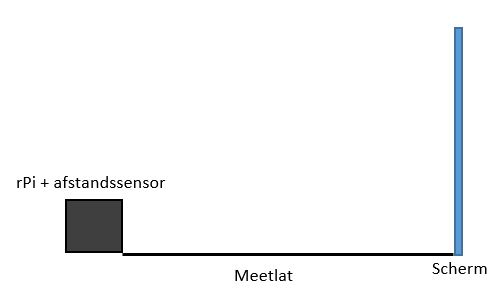
\includegraphics[scale=0.6]{opstelling.jpg}%
\caption{testopsteling}%
\label{opstelling}%
\end{figure}
\section{Verloop}
De test bestaat uit het meten van 11 verschillende afstanden (10, 20, 30, 60, 90, 100, 110, 120, 130, 140 en 150 cm). Deze zijn zo gekozen om meer kennis te hebben over kleine afstanden en over de verwachte vlieghoogte. Deze afstanden worden elk 500 keer gemeten, om de 60 ms. Deze waarden zijn zo gekozen, om toch voldoende nauwkeurigheid te hebben, veronderstellende dat er uitschieters zouden zijn. 

\section{Gegevens en verwerking}

Het uitvoeren van de testen nam per afstand gemiddeld 32 seconden in beslag. Omdat dit tijdens het opereren van de zeppelin onhaalbaar is, hebben we besloten om het interval te verlagen naar 10 ms. Zo kunnen de metingen zes keer zo snel gebeuren. 

Omdat 500 metingen nog steeds 6 seconden duren, hebben we het aantal verlaagd. We hebben d.m.v. rolling median de mediaan berekend van 10 en 20 opeenvolgende gegevens. Minder dan 10 is niet nauwkeurig genoeg, en voor meer dan 20 samples is de registratietijd te hoog. Uit deze gegevens hebben we om een aantal redenen besloten om een window van 10 samples te nemen.  Ten eerste is er de nauwkeurigheid als de zeppelin stijgt/daalt. Het hoogteverschil tussen sample 1 en 10 is immers kleiner dan dat tussen 1 en 20. Ten tweede is er de snelheid. Het spreekt voor zich dat het registreren van 10 samples minder lang duurt dan 20 samples. Tenslotte is er ook het minieme verschil tussen de gemiddelde mediaan bij 10 en 20 metingen. Minder metingen zorgen dus voor een even grote nauwkeurigheid. 

Een nadeel is wel dat de standaardafwijking van de medianen bij een breedte van 10 samples gemiddeld 0.2 cm groter is dan bij 20 samples. Dit weegt echter niet op tegen de winst aan snelheid en nauwkeurigheid.\\ 

Voor de meetgegevens: zie onderstaande tabel. \\

\begin{tabular}{r||r|r|r|r|r|r|r|r|r|r|r}
\textbf{Afstand} & 10 & 20 & 30 & 60 & 90 & 100 & 110 & 120 & 130 & 140 & 150 \\
\hline \hline 
$\mu$ (med.) (10) & 10.8 & 20.5 & 30.8 & 58.0 & 88.3 & 98.7 & 108.5 & 117.3 & 127.74 & 137.0 & 147.10 \\
$\mu$ (med.) (20) & 10.8 & 20.7 & 30.7 & 58.0 & 88.3 & 98.7 & 108.5 & 117.3 & 127.7 & 137.0 & 147.1 \\
$\sigma$ (med.) (10) & 0.21 & 0.52 & 0.82 & 0.55 & 0.70 & 0.72 & 0.68 & 0.94 & 0.58 & 0.60 & 0.69 \\
$\sigma$ (med.) (20)& 0.09 & 0.33 & 0.71 & 0.41 & 0.59 & 0.56 & 0.47 & 0.54 & 0.43 & 0.37 & 0.49 \\
\end{tabular}
\section{Conclusie}
De afstandsmeter meet het meest nauwkeurig bij kleine afstanden, bij grotere afstanden (meer dan 60 cm) liggen de meetresultaten gemiddeld iets onder de opgelegde afstand. Relatief gezien blijft de fout nog klein en kunnen we deze afwijking in het vervolg incalculeren bij het bepalen van de meetwaarden. De afstandssensor geeft telkens de mediaan van 10 gegevens door volgens het principe van de “rolling median”-techniek. Tien gegevens zorgen voor voldoende nauwkeurigheid, maar hebben ook het aspect dat de mediaanberekeningen snel genoeg gebeuren. Tevens is dit bij een hoogteverandering accurater. Deze methode boet wel in op de standaardafwijking. De gegevens wijken dus meer uit, maar dit weegt niet op tegen de voorgenoemde pluspunten. Om de afstandsregistratie nog sneller te laten verlopen, meet de afstandsmeter om de 10 ms. Een vertraging van 32 seconden is niet acceptabel.

\end{document}
